%
%
%

\section{Case Study: High-Payload Parallel Robot for Naval Experiments}
\label{sec:eval_water}


%

%

%

%
%
%
%
%
%
%
%
%
%
%
%

In this section, the synthesis framework is applied to a task requiring high payloads with high additional external and inertial forces. %
%
%
A naval testbed from the Ludwig Franzius Institute of Hydraulic, Estuarine, and Coastal Engineering (LuFI) at the Leibniz University Hannover (LUH) shall be equipped with a six-DoF parallel robot to measure external hydrodynamic forces during forced motion of mooring systems or ship models.
The task is introduced in Section~\ref{sec:eval_lufi_intro}, detailed in Section~\ref{sec:eval_lufi_task}, and transferred to the synthesis framework in Section~\ref{sec:eval_lufi_synthesis}.
The results are shown in Sections~\ref{sec:eval_lufi_results} and \ref{sec:eval_lufi_engsol}, in Appendix~\ref{sec:app_lufipkm}, and summarized in Section~\ref{sec:eval_lufi_summary}.
A hexapod-robot prototype was constructed based on the results within the thesis \cite{Fettin2023_M1174}. %

\subsection{Introduction and Related Work}
\label{sec:eval_lufi_intro}

Tasks that require high payloads and a limited range of motion are predestined for \propername{Gough}--\propername{Steward}-type parallel robots, such as flight simulators or devices for applying forces on mechanical parts in multiple directions (e.g., historically for tire testing) \cite{Merlet2006}. 
\emph{Devices for moving attached objects} within water or wind belong to the latter category.
They are required for identifying parameters and validating (numerical) fluid-dynamics models (e.g., from computational fluid dynamics or lumped-parameter models). 
This, combined with additional end-effector force measurements, helps improve simulations and the hydrodynamic or aerodynamic design of structures \cite{GibertiFer2015}.
%

The 6-\underline{P}US %
%
structure with parallel coplanar rails (HexaGlide) from a milling machine was chosen for moving a down-scaled model for flying objects within a \emph{wind tunnel} \cite{Bergmann2005}, termed ``model-positioning mechanism''.
The dimensional synthesis of different (non-parallel) rail alignments of the 6-\underline{P}US (then termed HexaSlide) was, e.g., investigated in \cite{RaoRaoSah2005} in a multi-objective optimization using SQP.
This was taken on by \cite{GibertiFer2015} to design a hybrid testbed for hardware-in-the-loop simulation of water-floating structures in a wind tunnel.
The dimensional synthesis based on a single-objective GA showed better performance in that task for the HexaSlide than the hexapod \cite{FioreGib2016} or HexaGlide \cite{GibertiLaResPar2018}.

In contrast to the wind tunnel, the installation space for a sole \emph{hydrodynamic testbed} is less restricting, as free space exists above the water level, where the robot is mounted from above.
As a result, hexapods are used for multi-axis naval experiments such as forced-oscillations tests, which were, e.g., performed in \cite{ArinoWilRusGry2015} for the down-scaled model of a subsea blowout preventer using a specialized hexapod from Symétrie \cite{SymetrieHexapods}.
A similar parallel-robot setup for a wave basin %
%
%
at LUH's LuFI is subject to the following combined structural and dimensional synthesis since the optimal structure depends on the specific requirements at the site, and a custom solution was preferred.

\subsection{Task Description and Requirements}
\label{sec:eval_lufi_task}

The \emph{mechanical requirements} are defined by the dimensions of the cross-section of the \SI{110} m long basin, as shown in Figure~\ref{fig:lufipkm_task}a for the empty channel with a width of \SI{2.2} m, a height of \SI{2} m, a regular water depth of \SI{1.0} m, and waves with an amplitude of up to \SI{0.5} m.
The \emph{installation space} of the parallel robot above the basin's upper edge should be kept relatively small to simplify construction and operation, as an indoor crane can only partially reach the basin.
A safety margin of \SI{0.3} m is defined relative to the basin's walls, which leaves an allowed installation space with a width of \SI{1.6} m and a height of \SI{1.5} m above normal water level.
To avoid \emph{design} complications, the robot's moving parts should not pass the robot's base frame, which should be compatible with the geometry of the basin's upper edge.
Further, the robot shall also be used in an open wave basin at a second location of the LuFI and, therefore, has to be transportable, \hl{facing up and down}, and {be} easy to assemble. %
The open wave basin produces 3D waves, which are also taken into account for the force requirements.

\begin{figure}[H]
  \begin{adjustwidth}{-\extralength}{0cm}
    \centering
    \graphicspath{{Figures/}}
    \input{./Figures/lufipkm_task.pdf_tex}
  \end{adjustwidth}
  \caption[Wave basin, robot and ship model for the naval-testbed task]{Photograph of the LuFI wave basin with sketched dimensions (not true to scale) of the allowed robot installation space (green) and workspace (blue) (\textbf{a}), rendering of the robot (\textbf{b}) with detail on the end effector (\textbf{c}). Geometrical relations and perspectives are depicted qualitatively. Modified from \cite{Fettin2023_M1174}.}
  \label{fig:lufipkm_task}
\end{figure}

In operation, a \emph{ship model} (dimensions \SI{0.4} m, \SI{0.48} m, \SI{2.1} m, mass \SI{54.2} kg) with a T-beam mechanical interface is mounted at the robot's end effector as shown in Figure~\ref{fig:lufipkm_task}b,c, which exerts external forces and moments $\bm{w}_\mathrm{ext}$ by hydrostatic and hydrodynamic effects. 
The ship's center of mass lies in the origin of the end-effector frame $\ks{\indks{E}}$.
The interface forces are measured by a force-torque sensor mounted at the platform with frame $\ks{\indks{P}}$ shown in Figure~\ref{fig:lufipkm_task}c, which requires a platform diameter of at least \SI{80}{\milli\metre}.
%
The \emph{process requirements} are defined by the forced motion of the ship in waves with amplitudes up to \SI{25}{\milli\metre}.
The wave basin's full amplitude is not used due to the focus on forced oscillation and the down-scaled model.
Separate harmonic oscillations with a frequency of \SI{1.25}{\hertz} and amplitude of \SI{100}{\milli\metre} or \SI{15}{\degree} in all six DoFs are considered.
Based on existing hydrodynamic model parameters, the maximal values of the external force in this motion are used for the synthesis.
The respective maximal forces from different effects (i.e., wave force, forced oscillation, damping, hydrostatic forces) are superposed to obtain safe dimensioning.
The demanded \emph{accessible workspace} is defined as a cube with sides of \SI{200}{\milli\metre} to allow vertical or horizontal motion of $\pm{}$\SI{100}{\milli\metre} amplitude.
Within the position workspace, tilting and rotation angles \SI{15}{\degree} against the neutral (untilted) pose must be achievable.


%

%

%


\subsection{Transfer to the Combined Structural and Dimensional Synthesis}
\label{sec:eval_lufi_synthesis}

The task requirements from above are transferred to the proposed synthesis framework of Section~\ref{sec:materials}.
The constraints, parameters, and load details are summarized in Table~\ref{tab:lufi_constraints} with reference to the numbered lists in Section~\ref{sec:ds_constraints} (for constraints) and Section~\ref{sec:dimsynth_optvars} (for parameters).
Installation space (row~\refl{luficonstr:installspace}), %
%
base/platform diameters (rows~\refl{luficonstr:baselim} and~\refl{luficonstr:plflim}), and base position (row~\refl{luficonstr:baseposition_z}) can be taken from the requirements with minor adaptions.
Some parameters are not subject to optimization, such as the horizontal base position (row~\refl{luficonstr:baseposition_xy}, thereby maintaining a symmetric alignment) or the chosen platform adapter for the ship model (row~\refl{luficonstr:ee_translation}).
Only a vertical rotation of the base relative to the task (row~\refl{luficonstr:param_baseori}) and of the end effector relative to the platform (row~\refl{luficonstr:param_eeori}) is considered for optimization, not the tilting angles, to simplify manufacturing and assembly.
The payload and the worst-case external forces are given values (rows~\refl{luficonstr:payload_mass}--\refl{luficonstr:moments}).

The \emph{workspace requirements} are translated into 342 different poses (``reference points'') at 27 positions that sample the cube in steps of \SI{100}{\milli\metre}.
Each position is tested with varying combinations of $X$-$Y'$-$Z''$ \propername{Euler} angles for the end-effector frame, $\varphi_x,\varphi_y,\varphi_z \in \{\SI{-15}{\degree},\SI{0}{\degree},\SI{15}{\degree}\}$, similar to \cite{Kirchner2000} (p.\,126), leading to tilting angles of up to \SI{21}{\degree}.
To reduce the number of poses, symmetry of the workspace is assumed, and the full orientation variation is used only for outer points.
The \emph{reference trajectory} between {the 342 poses} has 7~k samples (with sampling time \SI{50}{\milli\second}, trapezoidal acceleration profile, $a_\mathrm{max}=$ \SI{3}{\metre\per\square\second}, and $v_\mathrm{max}=$\SI{1}{\metre\per\second}, chosen based on previous one-axis forced-oscillation experiments). %

A threshold for the robot \propername{Jacobian} condition number (row~\refl{luficonstr:condjac}) avoids structures with an unbalanced transmission ratio between the actuators and, therefore, asymmetric load.
The material stress of the robot links is checked without additional safety factors (row~\refl{luficonstr:materialstress}) since the assumed external forces already include a safety margin.
A link design optimization is performed to obtain a dimensioning that withstands the high loads.

The list of potential structures is not limited by specific design requirements. %
Therefore, all \PKMTTTRRRnumactuation{} of the 3T3R parallel robots from a structure database may be tested.
It is based on a geometric permutation of the alignment of base- and platform-coupling joints from Section~\ref{sec:dimsynth_optvars} and the leg chains of \cite{Ramirez2018}, which are based on the permutation of Denavit--Hartenberg parameters. %
Some structural filters are applied, nevertheless.
By using only active revolute first or second joints, larger motion of the electric motors, which are expected to be bulky regarding the payload, is avoided.
%

\newcounter{luficonstraints}
\begin{table}[H]
  \caption{Constraints and parameter limits for the naval-testbed task.} %
\label{tab:lufi_constraints}
\begin{adjustwidth}{-\extralength}{0cm}
  \centering
  \begin{tabularx}{\fulllength}{CcCc}
    \toprule
    \textbf{\#} & \textbf{Constraint} & \textbf{Section~\ref{sec:ds_constraints}} &  \textbf{Value} \\
    \midrule
    \refstepcounter{luficonstraints}\theluficonstraints\label{luficonstr:installspace} & installation space (see Figure~\ref{fig:lufipkm_task}) & no.~\refl{itm:constr_installspace} %
    %
    & max. width \SI{1.6} m, height \SI{1.5} m \\
    \midrule
    \refstepcounter{luficonstraints}\theluficonstraints\label{luficonstr:baselim} & base diameter & no.~\refl{itm:constr_param_radius}  &  800--1500 mm \\
    \midrule
    \refstepcounter{luficonstraints}\theluficonstraints\label{luficonstr:plflim} & platform diameter & no.~\refl{itm:constr_param_radius} &  200--800 mm \\	
    \midrule
    \refstepcounter{luficonstraints}\theluficonstraints\label{luficonstr:condjac} & \propername{Jacobian} condition number & no.~\refl{itm:constr_jac_traj} & max. 500 (mixed units) \\
    \midrule
    \refstepcounter{luficonstraints}\theluficonstraints\label{luficonstr:materialstress} & material stress & no.~\refl{itm:constr_materialstress} & max.~\SI{100}{\percent} (of yield strength)\\
    \midrule
    
    & \textbf{Parameter} & \textbf{Section~\ref{sec:dimsynth_optvars}} &  \textbf{Value} \\
    \midrule
    \refstepcounter{luficonstraints}\theluficonstraints\label{luficonstr:baseposition_z} & vertical base position in $\rovec{\indks{W}}{0}$ & no.~\refl{itm:param_basepos} & 1.1--2.5 m \\
    \midrule
    \refstepcounter{luficonstraints}\theluficonstraints\label{luficonstr:baseposition_xy} & base position in $x$-$y$-plane & no.~\refl{itm:param_basepos} & 0 (no optimization) \\
    \midrule
    \refstepcounter{luficonstraints}\theluficonstraints\label{luficonstr:param_baseori} & \gape{base rotation $\rotmat{\indks{W}}{0}$} & no.~\refl{itm:param_baseori} & $\varphi_{\mathrm{b},x}=\varphi_{\mathrm{b},y}=0$ and $\varphi_{\mathrm{b},z}\in [-\SI{180}{\degree},\SI{180}{\degree}]$\\
    \midrule
    \refstepcounter{luficonstraints}\theluficonstraints\label{luficonstr:ee_translation} & end-effector translation $\rovec{\indks{P}}{\indks{E}}$ & no.~\refl{itm:param_eepos} & [0,\,0,\,200] \SI{}{\milli\metre} (schematic in Figure~\ref{fig:lufipkm_task}) \\	
    \midrule
    \refstepcounter{luficonstraints}\theluficonstraints\label{luficonstr:param_eeori} & \gape{end-effector rotation $\rotmat{\indks{P}}{\indks{E}}$} & no.~\refl{itm:param_eeori} & $\varphi_{\mathrm{p},x}=\varphi_{\mathrm{p},y}=0$ and $\varphi_{\mathrm{p},z}\in [-\SI{180}{\degree},\SI{180}{\degree}]$\\
    \midrule
    & \textbf{Load} &  &  \textbf{Value} \\
    \midrule
    \refstepcounter{luficonstraints}\theluficonstraints\label{luficonstr:payload_mass} & payload mass (ship hull) &  &  \SI{54.2} kg \\	
    \midrule
    \refstepcounter{luficonstraints}\theluficonstraints\label{luficonstr:payload_inertia} & \gape{payload inertia $\ortvek{\indks{P}}{I}{(\point{C}_\mathrm{P})}{}$} &  & $[I_{xx},I_{yy},I_{zz}]=$ [0.4,\,8.3,\,8.3] \SI{}{\kilo\gram\metre\squared} \\
    \midrule
    \refstepcounter{luficonstraints}\theluficonstraints\label{luficonstr:forces} & maximal external forces &  &  \gape{$\ortvek{\indks{W}}{f}{\transp}{\mathrm{ext}}=$ [34,\,451,\,659] \SI{}{\newton}} \\
    \midrule
    \refstepcounter{luficonstraints}\theluficonstraints\label{luficonstr:moments} & maximal external moments &  & \gape{$\ortvek{\indks{W}}{m}{\transp}{\mathrm{ext}}=$[67,\,608,\,162] \SI{}{\newton\metre}} \\
    \bottomrule
  \end{tabularx}
\end{adjustwidth}
\end{table}

In summary, nearly six thousand different structure variants are considered due to the high number of base- and platform-coupling joint alignment combinations as discrete design parameters.
For each variant, a PSO is performed on the LUH computing cluster~\cite{LUISCLUSTER}, using 100 iterations and 200 individuals in multiple subsequent trials, where the initial values are obtained partly random, partly from previous results.
Parameters from different coupling-joint alignments of a variant are also transferred between the consecutive trials to increase the population's diversity.
The optimization was aborted after two to eight hours as this led to adequately feasible solutions for iteratively adjusting the settings.
The computation time per particle is about \SI{60}{\second} if no early abortion occurs.
If multiple assembly modes are valid, the time further increases to evaluate all and find the best one.
%
The number of optimization variables is up to 21, depending on the structure.


\subsection{Synthesis Results for the Naval-Testbed Robot}
\label{sec:eval_lufi_results}

%
%
%
%
%

The link design optimization is first omitted to investigate its necessity.
Objectives for the mechanical design of the robot are evaluated for an initial estimate of possible solutions.
The objectives are the collision distance (objective \refl{itm:obj_colldist} from Section~\ref{sec:ds_objective}) and the material stress (obj.~\refl{itm:obj_materialstress}) for the relatively lightweight default link dimensioning (hollow cylinder with \SI{13}{\milli\metre} diameter, \SI{1}{\milli\metre} strength).
The stress limit (row \refl{luficonstr:materialstress} in Table~\ref{tab:lufi_constraints}) is ignored at this stage.
The \propername{Pareto} diagram in Figure~\ref{fig:lufipkm_pareto_materialstresscolldist_34joints} summarizes the results for structures with three and four joints in the leg chains.
Results for five and six joints are within appendix Figure~\ref{fig:lufipkm_pareto_materialstresscolldist_56joints}.
From the diagrams, it becomes clear that the high payload and external forces produce significant material stress, which can be held well by rod kinematics like the hexapod %
%
(\hyperrefl{restabrow:P6RRPRRR14V6GxPxA3}{6-U\underline{P}S}, Figure~\ref{fig:lufipkm_robots1}a), its kinematic inversion (\hyperrefl{restabrow:P6RRRPRR9V9GxPxA4}{6-S\underline{P}U}, Figure~\ref{fig:lufipkm_robots1}b), or variants of the two (\hyperrefl{restabrow:P6RRPRRR14V5GxPxA3}{6-{R}{R}\underline{P}{S}} in Figure~\ref{fig:lufipkm_robots1}c and \hyperrefl{restabrow:P6RRRPRR9V8GxPxA4}{6-{U}{R}\underline{P}{U}} in Figure~\ref{fig:lufipkm_robots1}d).
Other feasible structures are another \hyperrefl{restabrow:P6RRRPRR15V8GxPxA4}{6-{U}{R}\underline{P}{U} variant}  (Figure~\ref{fig:lufipkm_robots3}i) or the 6-{R}{U}\underline{P}{U} (Figure~\ref{fig:lufipkm_robots1}e or Figure~\ref{fig:lufipkm_robots3}c) with short levers.
Parallel robots %
%
with the same joint order can differ by the parallelism of their joints or additional skew angles, visible in the Denavit--Hartenberg parameters given in the tables in Appendix~\ref{sec:app_lufipkm}.
The kinematic inversions (e.g., 6-S\underline{P}U instead of 6-U\underline{P}S) were investigated since R, U, and S joints have different ranges of motion.
The geometric dimensioning of the robot then has to be different, which is visible in the lower performance of the 6-S\underline{P}U.
Other structures exceed the material-stress limit and require stronger dimensioning of the links by the design-optimization loop, which is included in the following.
\vspace{3pt}
\begin{figure}[H]
\begin{adjustwidth}{-\extralength}{0cm}
  \centering
  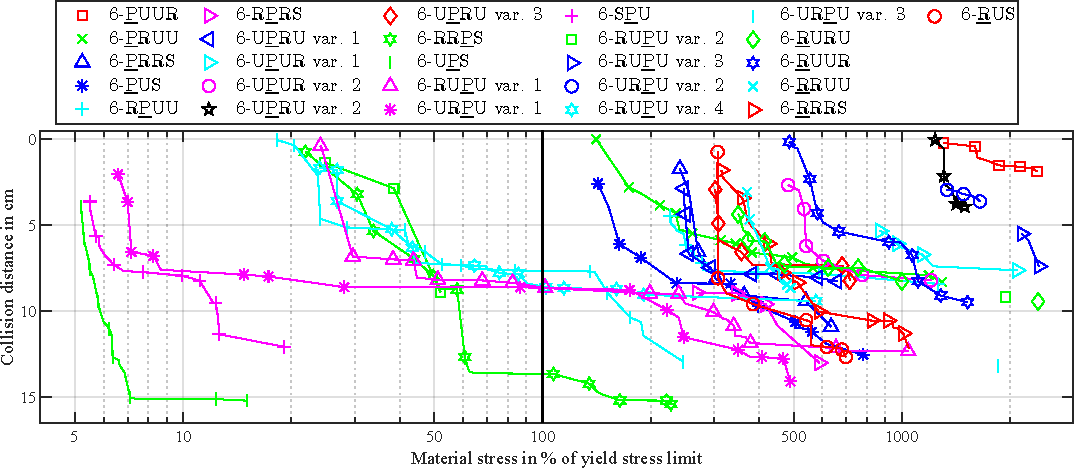
\includegraphics{Figures/lufipkm_pareto_materialstress_colldist_groups_materialstresscolldist_34joints.pdf}
\end{adjustwidth}
\caption[Naval-testbed task: \propername{Pareto} fronts for design-oriented objectives for chains with three and four joints]{\propername{Pareto} fronts for design-oriented objectives for chains with three and four joints with lightweight link dimensioning without the link-design optimization loop.}
\label{fig:lufipkm_pareto_materialstresscolldist_34joints}
\end{figure}

\vspace{-12pt}
\begin{figure}[H]
\begin{adjustwidth}{-\extralength}{0cm}
  \centering
  \graphicspath{{Figures}}
  \input{./Figures/lufipkm_robots1.pdf_tex}
\end{adjustwidth}
\caption{Visualization %
  %
  of valid solutions for the naval-testbed robot from Figure~\ref{fig:lufipkm_pareto_materialstresscolldist_34joints}. The fixed base is at the top, and the moving platform is at the bottom. Red cuboids mark active prismatic joints, and blue cylinders or spheres mark passive joints.}
\label{fig:lufipkm_robots1}
\end{figure}

%
In another run of the optimization, the objectives were selected as the  moving parts' mass (excluding motors and joints, objective~\refl{itm:obj_mass} from Section~\ref{sec:ds_objective}), the actuators' rated power (obj.~\refl{itm:obj_power}), and again, the collision distance (obj.~\refl{itm:obj_colldist}).
Figure~\ref{fig:lufipkm_pareto_power_mass_groups_default_hexapod_and_hexa} shows the \propername{Pareto} diagrams of the first two objectives for the combination of base- and platform-joint alignments for a hexapod (a), a Hexa (b), and a HexaSlide~(c).
The mass is influenced mainly by the length of the links and the force distribution within the structure, as high material stress (resulting from bending moments from levered forces) requires stronger dimensioning.
The Hexa and the HexaSlide have higher stress in Figure~\ref{fig:lufipkm_pareto_materialstresscolldist_34joints}, and also, after the design optimization, a higher moving structural mass than the hexapod.
However, no dominant structure can be stated regarding the neglected mass of the hexapod's moving actuators and the mass difference of less than 10\% (regarding \SI{60} kg).
\begin{figure}[H]
\begin{adjustwidth}{-\extralength}{0cm}
  \centering
  \begin{overpic}
  {Figures/lufipkm_alignment_compare_RUS_UPS.pdf}
  \put(0,1){(\textbf{a})}
  \put(34,1){(\textbf{b})}
  \put(67,1){(\textbf{c})}
  \end{overpic}  
\end{adjustwidth}
\caption{\propername{Pareto} fronts
  for combinations of coupling-joint alignments of selected parallel robots: (\textbf{a}) Hexapod, (\textbf{b}) Hexa, and (\textbf{c}) HexaSlide}
\label{fig:lufipkm_pareto_power_mass_groups_default_hexapod_and_hexa}
\end{figure}

Performing the dimensional synthesis for several coupling-joint alignments without preliminary fixing allows for comparing their performance.
The HexaGlide discussed in Section~\ref{sec:eval_lufi_intro} (6-\underline{P}US with parallel horizontal base coupling, ``p'') does not provide any solutions due to collisions and the limited available installation space.
The actuator's rated power is approx. 20\% lower for the hexapod (\SI{800}{\watt} compared to \SI{1}{\kilo\watt}).
Since a spherical joint is used for the platform joints of the three structures, only pairwise and regular circular distributions are distinguished with two colors in Figure~\ref{fig:lufipkm_pareto_power_mass_groups_default_hexapod_and_hexa}, in contrast to the base joints with nine possible markers.
The pairwise alignment of both base and platform joints (shifted by one) outperforms other possible alignments for all structures.
Thereby, the optimization algorithm obtains the established alignments from the literature without prior specific knowledge, showing the feasibility of the permutational approach for parallel\hl{-}robot synthesis.


Next, all robot structures are compared regarding the three criteria relevant to the mechanical design and technical realization, summarized in the two \propername{Pareto} diagrams in Figure~\ref{fig:lufipkm_pareto_power_mass_groups}.
Only the \propername{Pareto}-dominant coupling-joint alignments are included, as well as the custom hexapod engineering solution from \cite{Fettin2023_M1174} (see Section~\ref{sec:eval_lufi_engsol}) based on the synthesis.
By comparing moving mass and actuator power (upper part in Figure~\ref{fig:lufipkm_pareto_power_mass_groups}), the same robot assemblies as in Figure~\ref{fig:lufipkm_pareto_materialstresscolldist_34joints} are dominant since the necessary stronger link dimensioning of the previously underdimensioned structures increases their mass.
Most of these structures lead to valid solutions, meaning that the link-design optimization found a stronger dimensioning that was also free of self-collisions despite the increased link~diameters.
The total of 40 structures are listed in Figure~\ref{fig:lufipkm_pareto_power_mass_groups}%
%
, as opposed to 26 in Figure~\ref{fig:lufipkm_pareto_materialstresscolldist_34joints} and \hl{17} in Figure~\ref{fig:lufipkm_pareto_materialstresscolldist_56joints}, with only a few with stress below 100\%. %

The collision criterion is investigated in the lower part of Figure~\ref{fig:lufipkm_pareto_power_mass_groups}.
The dominance of the hexapod becomes visible for this task, as {it} provides the largest possible distances between the leg chains due to its compact construction.
This also presents a safety margin for motion outside of the prescribed workspace and leaves room for detailed construction since collision bodies for the actuators are not included in the simplified model in the synthesis.
For the design of the system, not only the actuators' rated power but also their torque and speed have to be compared to select from catalogs of existing motor-gear combinations.
Together with the collision distance, these objectives (numbers~\refl{itm:obj_maxactforce} and \refl{itm:obj_maxactvelo} in Section~\ref{sec:ds_objective}) were optimized in another run, resulting in \propername{Pareto} diagrams in \mbox{Figures~\ref{fig:lufipkm_pareto_linkdiam_colldist}--\ref{fig:lufipkm_pareto_motordiagram_revolute}} in the appendix.
For prismatic actuation, these drive-train characteristics constitute one dense \propername{Pareto} front, showing an equivalence of most structures regarding these criteria, which does not hold for revolute actuation.
The stronger dimensioning of some of the structures as \hl{the} result of the design optimization is visible as well (Figure~\ref{fig:lufipkm_pareto_linkdiam_colldist} and Tables~\ref{tab:lufipkm_results_pris} and~\ref{tab:lufipkm_results_rev}). %
Further robot sketches (Figures~\ref{fig:lufipkm_robots2}--\ref{fig:lufipkm_robots4}) and tables with characteristic values and dimensional parameters (Tables~\ref{tab:lufipkm_results_pris}--\ref{tab:lufipkm_results_rev_dh}) are given in Appendix~\ref{sec:app_lufipkm} for compactness.

\begin{figure}[H]
\begin{adjustwidth}{-\extralength}{0cm}
  \centering
  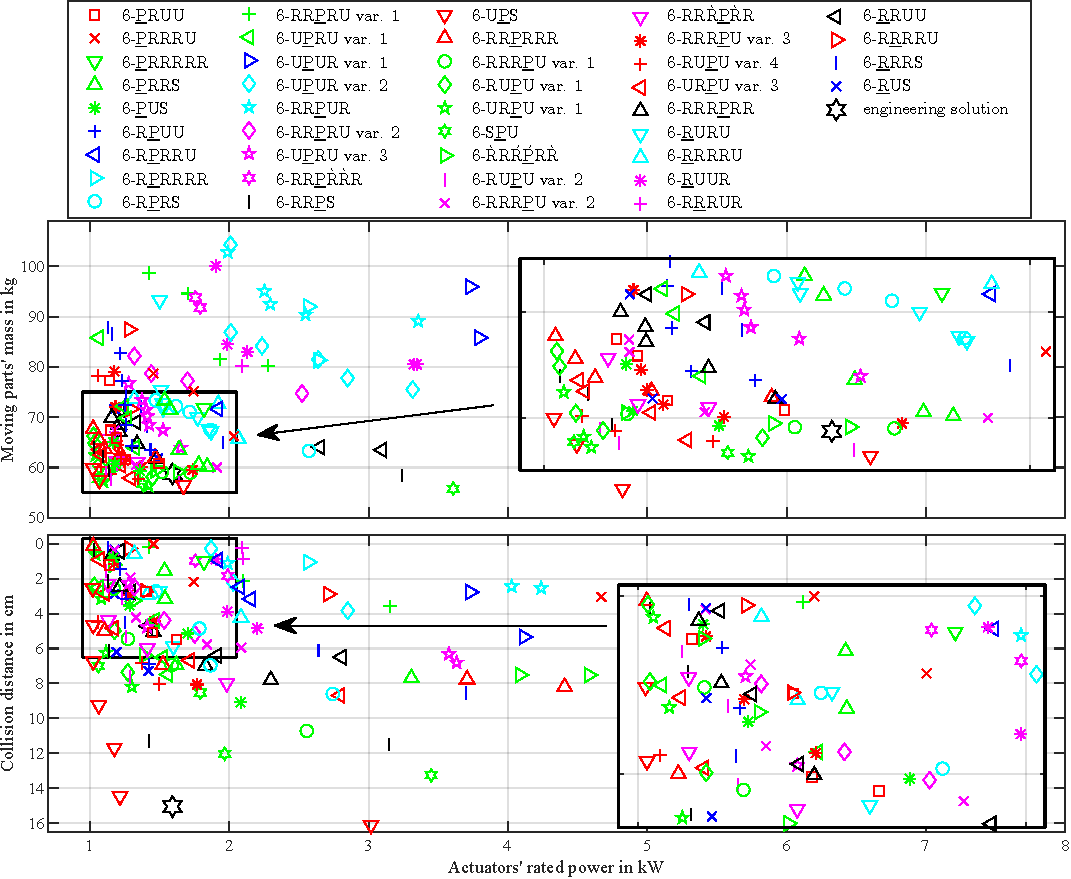
\includegraphics{Figures/lufipkm_pareto_3obj_combined.pdf}
\end{adjustwidth}
\caption{Grouped \propername{Pareto} fronts of all results of the naval-testbed robot.}
\label{fig:lufipkm_pareto_power_mass_groups}
\end{figure}

\subsection{Engineering Solution}
\label{sec:eval_lufi_engsol}

A hexapod was selected in \cite{Fettin2023_M1174} as the most feasible solution for the task.
The final dimensioning was determined based on several runs of the dimensional synthesis and as a compromise solution for multiple objectives (force, velocity, collision, precision, workspace, stiffness, workspace size) and computed for the 3D \propername{Pareto} front of the synthesis with objectives of force, velocity, and collision distance.
The workspace volume was evaluated by a discretization approach from \cite{TartariFilhoCab2005,GharahsoflooRah2015}, which is not feasible to be performed within the dimensional synthesis due to the computation time. 
The objectives were normalized to their best possible value and weighted using a paired comparison based on economic, practical, and task considerations.
Therefore, the solution is not dominant in Figures \ref{fig:lufipkm_pareto_power_mass_groups}, \ref{fig:lufipkm_pareto_motordiagram_prismatic}, and \ref{fig:lufipkm_pareto_motordiagram_revolute}, {i.e., it is above the \propername{Pareto} front for the 6-U\underline{P}S.}
An overview of the resulting construction is given in Figure~\ref{fig:lufipkm_engineering}.
The geometric parameters and performance characteristics are shown in the last row of appendix Table~\ref{tab:lufipkm_results_pris}, together with values for other structures.

\vspace{-2pt}
\begin{figure}[H]
\begin{adjustwidth}{-\extralength}{0cm}
  \centering
  \graphicspath{{Figures}}
  \input{./Figures/lufipkm_engsol.pdf_tex}
\end{adjustwidth}
\caption{\hl{Details} of the engineering solution; modified from \cite{Fettin2023_M1174}: (\textbf{a}) leg chain (modified from the catalog ``Electromechanical cylinders EMC'' from Bosch Rexroth AG, Lohr am Main, Germany), (\textbf{b}) spherical joint, (\textbf{c}) universal joint (derived from a CAD file of Elso Elbe GmbH \& Co. KG., Hofheim, Germany), (\textbf{d}) hexapod assembly, (\textbf{e}) moving platform, and (\textbf{f}) fixed base.} %
\label{fig:lufipkm_engineering}
\end{figure}

The found structure (cf. Figure~\ref{fig:lufipkm_engineering}d) is a classical hexapod with pairwise alignments of base- and platform-coupling joints with correspondence shifted by one.
%
Electric lifting cylinders based on a spindle and axis-parallel motor alignment  (cf. Figure~\ref{fig:lufipkm_engineering}a) were used directly for the leg chains, dimensioned regarding the minimal and maximal stroke and the required actuator force and speed from the simulation.
Further specific constraints had to be respected (i.e., inability to use the full stroke under load, cylinder length offset to account for joint and adapter dimensions, and ability to support the total system's mass when the robot stands on the mobile platform).
The same standard universal joints (cf. Figure~\ref{fig:lufipkm_engineering}c) were used for the base and platform coupling due to their availability.
An additional revolute joint was added for the kinematic spherical joint (cf. Figure~\ref{fig:lufipkm_engineering}b), and no ball-and-socket joints were used.
%
A tilt adapter for the base- and platform-coupling joints (cf. \SI{21.5}{\degree} in Figure~\ref{fig:lufipkm_engineering}e) was chosen to reduce the joints' tilting angle to \SI{31}{\degree} (of maximal \SI{35}{\degree}) during the reference motion.
The base-frame design (Figure~\ref{fig:lufipkm_engineering}f) fulfills the requirements regarding interface compatibility, transportability, and parts availability.

The mechanical design of the base showed that the resulting parameter for base-rotation offset is not feasible, and a parallel alignment of one base-joint pair to the frame's edge by $\varphi_{\mathrm{b},z}{=}\SI{180}{\degree}$ was used instead (Figure~\ref{fig:lufipkm_engineering}f), which only led to negligible degradation of the system performance.
The same holds for the platform rotation offset parameter $\varphi_{\mathrm{p},z}$, which now can be set in discrete values of \SI{15}{\degree} with the circular flange  (Figure~\ref{fig:lufipkm_engineering}e) and makes the robot adaptable to different tasks and ship models.


\subsection{Summary of the Case Study}
\label{sec:eval_lufi_summary}


%
%
%
%
%
%

For the naval-testbed task, the combined structural and dimensional synthesis found valid solutions for the majority of available kinematic structures.
The best performance of the design-oriented objectives was achieved by widely-used structures with three joints per chain.
For these standard solutions (see, e.g., \cite{FrindtKreHes2010}), the framework presents an efficient approach for dimensional synthesis.
%
Other solutions were not able to outperform the standard designs. 
The reasons are the rather nonrestrictive ratio of workspace to installation space and the moderate required tilting angles already achievable by the hexapod. %
Furthermore, the payload produces high bending moments for structures with multiple joints and longer~levers.
%

However, results for structures with more joints are still feasible regarding their performance despite their high design complexity.
The acceptable computational effort shows the \emph{feasibility of the approach for the link-design optimization}, which had to be employed for the multi-joint leg chains to obtain valid solutions.
%
The case study further indicates that after some iterations of the requirements and the synthesis results, the kinematic structure and the drive characteristics were a helpful basis for the design and construction of a robot prototype within the time limitation of a master's thesis.

%
%
%
%

After exploring the diversity of parallel robots with 3T3R end-effector DoFs that the proposed synthesis framework can produce, the subsequent case study focuses on robots with reduced mobility and functional redundancy. An example of using functional redundancy with 3T3R robots with the framework is given in \cite{SterneckFetSch2023}.
